

\documentclass[12pt]{extarticle} % set to 12 when done

\usepackage{outlines}
\usepackage{graphicx} % Add pictures to your document
\usepackage{listings} % Source code formatting and highlighting
\usepackage{amsmath}
\usepackage{amsthm}
\usepackage{extsizes}
\usepackage{amsfonts} 

\usepackage[margin=0.5in]{geometry}


\graphicspath{ {./pics/} }


\begin{document}
\newcommand\abs[1]{\left|#1\right|} % absolute
\newcommand\magnitude[1]{\left\Vert #1 \right\Vert}
\newcommand\vectoo[1]{\begin{bmatrix} #1 \end{bmatrix}}
\newcommand{\seq}[2][0]{\left\{ #2 \right\}_{n=#1}}
% ^ newcommand, use like \seq[startingg_n]{sequence}
\newtheorem{theorem}{Theorem}
\newtheorem*{theorem*}{Theorem}
\newtheorem*{definition}{Definition}

\section{Chapter 1, vector mathematics}

\subsection*{dot product}
The dot product is the product of 2 vectors, and produces a scalar.
$$
\vec{A} \cdot \vec{B} = \vectoo{a_1 \\ a_2} \cdot \vectoo{b_1 \\ b_2}
$$
My calc does it with A dot B

\subsection*{cross product}
Projecting A onto B : 
$${ \vec{A} \cdot \vec{B} \over \magnitude{\vec{A}}}$$


The Cross product of 2 linearly independent vectors (denoted like $\vec{A} \times \vec{B}$ ) results in a vector that's
perpendicular. 
It is \textbf{anti}commutative ($a \times b = - b \times a$) and distributive ( $a \times (b + c ) = a \times b + a \times c$ ). \\
Also, $a \times (b \times c) \not= (a \times b) \times c$ but i forgot the name of that.
To calculate it, do the following:
$$
\vec{a} \times \vec{b} = \hat{x} (a_y b_z - a_z b_y) + \hat{y} (a_z b_x - a_x b_z)  + \bar{z} ( a_x b_y - a_y bx)
$$

To get the angle between $\vec{a} \times \vec{b} = asin \left( a \times b \over \magnitude{a} \magnitude{b}  \right)$

\subsection*{Just review how to switch between cylindrical, spherical and rectangular coordinates}

$$
\begin{aligned}
    \text{del or nabla (gradient): } \nabla f &= \hat{x} {\partial f \over \partial x} 
+ \hat{y} {\partial f \over \partial y} + \hat{z} {\partial f \over \partial z} \\
\text{divergence of a} \nabla \vec{A} &= {\partial A_x \over \partial x} 
+ {\partial A_y \over \partial y} + {\partial A_z \over \partial z} \\
\text{curl of } \vec{A} : \nabla \times \vec{A} &=  \hat{x} ({\partial A_z \over \partial y} - {\partial A_y \over \partial z}) + 
\hat{y} ({\partial A_x \over \partial z} - {\partial A_z \over \partial x}) +
\hat{x} ({\partial A_x \over \partial y} - {\partial A_y \over \partial x}) 
\end{aligned}
$$

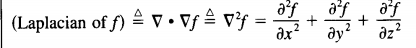
\includegraphics{1}

\newpage
\section{Charge, charge densities, coulomb's law, electric field intensity}
The smallest possible charge is the charge of an electron, $q_e = -1.6 \cdot 10^{-19}$ C
The unit for charge is C, the coulomb.

Charges are found on 
\begin{enumerate}  
    \item a point 
    \item a line
    \item a surface
    \item a volume
    \item a combination of the abovementioned
\end{enumerate}

A line charge on a length $\Delta l$ contains charge $\Delta Q$
The charge density can be defined as follows
$$
\rho_x = \lim_{x \rightarrow 0} {\Delta Q \over \Delta x } {C\over m^n} \text{a.a.p.}
$$
n is the dimensionality for line, surface, volume.
a.a.p. is at a point.

Furthermore, 
$$
Q_x = \int_x \rho_x dx
$$
where x is l,s,v. Plus, it's single, double and triple integrals respectively.

\subsection*{Force between charges}
charges have an effect on each other. If both are positive or negative, they repel each other,
and if they have opposite charges, they attract one another.
To calculate the force a charge has on another charge, we use this:

$$
\begin{aligned}
    \text{The force on Q1 by Q2} \\
    F_{12} =  { Q_1 \cdot Q_2 \cdot \hat{a}_{R_{12}} \over 4 \pi \cdot \epsilon_0 \cdot R_{12}^2} = 
    {Q_1 \cdot Q_2 \cdot \vec{R}_{12} \over 4 \pi \epsilon_0 \cdot R_{12}^3} newton, \\
    \text{where: } \\
    \hat{a}_{R_{12}} = \text{unit vector fromQ1 to Q2} = {R \over \magnitude{R}} \\
    \epsilon_0 = \text{ permitivity of free space } = {1\over 36 \pi} \cdot 10^{-9} {F \over m}  
\end{aligned}
$$

$F_{12} = - F_{21}$, because $\hat{a}_{R_{12}} = - \hat{a}_{R_{21}}$

The total force on a charge from other charges is the summation of all those forces.

\subsection*{2.4 Electric field intensity of point charges}

$F_{xy}$ is dependent on the location of charge $Q_x$, so it might be more appropriate to call it a vector force field.

$F_{xy}$, the vector electric field density at location of Q1, is the vector force field dividen by Q1, and can be calculated like so:

$$
E_x = {\vec{F}_x \over Q_x} = {Q_1 \hat{a}_{r_{12}} \over 4 \pi \cdot \epsilon_0 \cdot R_{1x}^2}
= = {Q_1 \vec{R}_{1x} \over 4 \pi \cdot \epsilon_0 \cdot R_{1x}^{3/2}}
$$

\subsection*{2.5 Electric field intensity of a line charge}
To evaluate the electric fielf from a line-, surface-, or volume charge, we do this:

$$
dE = {dQ \hat{a}_r \over 4 \pi cdot \epsilon_0 \cdot R^2} =
{ \rho_l d_l \hat{a}_r \over 4 \pi cdot \epsilon_0 \cdot R^2}
$$

$$
E = \int_a^bdE = \int_a^b { \rho_l d_l \hat{a}_r \over 4 \pi cdot \epsilon_0 \cdot R^2}
$$




\end{document}









